% !TEX program = lualatex 

\documentclass[9pt]{beamer}

\usetheme{metropolis}
\usepackage{bookmark}
\usepackage{xcolor-solarized}

\setbeamercolor{normal text}{%
  fg=solarized-base02,
  bg=solarized-base3!20!white
}
\setbeamercolor{alerted text}{%
  fg=solarized-red
}
\setbeamercolor{example text}{%
  fg=solarized-green
}
\setbeamercolor{frametitle}{%
    fg=solarized-blue!70!black,
    bg=solarized-base2
}

\setbeamerfont{title}{series=\bfseries,parent=structure}
\setbeamerfont{frametitle}{series=\bfseries,parent=structure}
\renewcommand{\footnotesize}{\scriptsize}
% sort
\newcommand{\issortedany}{\term{in-image}}
\newcommand{\issorted}{\issortedany_s}
\newcommand{\isheadleast}{\term{image-respects-pair}}
\newcommand{\istailsort}{\term{image-can-induct}}
\newcommand{\setord}{\term{Ord}}
\newcommand{\Ord}{\term{Ord}}
\newcommand{\setmtol}{\term{M2L}}
\newcommand{\setsort}{\term{Sort}}
\newcommand{\Sort}{\term{Sort}}
\newcommand{\otof}{\term{o2f}}
% constructions
\newcommand{\List}{\term{List}}
\newcommand{\Array}{\term{Array}}
\newcommand{\PList}{\term{PList}}
\newcommand{\SList}{\term{SList}}
\newcommand{\Bag}{\term{Bag}}
\newcommand{\Perm}{\term{Perm}}


\usecolortheme{orchid}

\usepackage{hott}
\usepackage{mathtools}
\usepackage{macros}
\usepackage[final]{microtype}

\usepackage{mathpartir}
\usepackage{worldflags}
\usepackage{stmaryrd}
\usepackage{lipsum}
\usepackage{adjustbox}
\usepackage{amsmath}
\usepackage{amssymb}
\usepackage{geometry}
\usepackage{mathrsfs}
\usepackage{braket}
\usepackage{quiver}
\usepackage{mathtools}
\usepackage{commath}
\usepackage{xparse}
\usepackage{array}
\usepackage{subcaption} %side by side diagrams
\usepackage{floatrow}
\usepackage{tikz}
\usepackage{tikz-cd}
\usetikzlibrary{babel}% added

% bibliography
\usepackage[style=authortitle,backend=biber]{biblatex}
\addbibresource{../../symmetries.bib}

% fancy boxes
\usepackage[most]{tcolorbox}

\newtcolorbox{qblock}[1][Question]{
  colback=white,
  colframe=solarized-orange,
  colbacktitle=white!90!structure.fg,
  coltitle=black,
  fonttitle=\itshape,
  title={#1},
  enhanced,
  attach boxed title to top left={yshift=-0.1cm, xshift=0.5em}
}
\newtcolorbox{dblock}[1][Definition]{
  colback=white,
  colframe=solarized-violet,
  colbacktitle=white!90!structure.fg,
  coltitle=black,
  fonttitle=\itshape,
  title={#1},
  enhanced,
  attach boxed title to top left={yshift=-0.1cm, xshift=0.5em}
}

\newtcolorbox{pblock}[1][Proposition]{
  colback=white,
  colframe=solarized-blue,
  colbacktitle=white!90!structure.fg,
  coltitle=black,
  fonttitle=\itshape,
  title={#1},
  enhanced,
  attach boxed title to top left={yshift=-0.1cm, xshift=0.5em}
}

\newtcolorbox{tblock}[1][Theorem]{
  colback=white,
  colframe=solarized-green,
  colbacktitle=white!90!structure.fg,
  coltitle=black,
  fonttitle=\itshape,
  title={#1},
  enhanced,
  attach boxed title to top left={yshift=-0.1cm, xshift=0.5em}
}

\usepackage{tikz}
\usetikzlibrary{cd}
\usetikzlibrary{fit}

\usepackage{fontspec}
\setmonofont{Iosevka}[
    Path=./Iosevka/,
    Extension = .ttf,
    UprightFont=*-Regular,
    BoldFont=*-Bold,
    ItalicFont=*-Italic,
    BoldItalicFont=*-BoldItalic
]

%Information to be included in the title page:
\title{Order from sorting with universal algebra}
\author[shortname]{
  Wind Wong \inst{1}
  \and Vikraman Choudhury \inst{2}
  \and Simon J. Gay \inst{1}
}
\institute[shortinst]{\inst{1} University of Glasgow \and %
                      \inst{2} Universit\`{a} di Bologna and OLAS Team, INRIA}
\date{February 14, 2024}

\begin{document}

\frame{\titlepage}

\begin{frame}
  \frametitle{Introduction}

  
  Consider a puzzle about sorting,
inspired by Dijkstra's Dutch National Flag problem~\footcite{dijkstraDisciplineProgramming1997}.
Suppose there are balls of three colors,
corresponding to the colors of the Dutch flag: red, white, and blue.
\[
  \{
  \tikz[anchor=base, baseline]{%
    \foreach \x/\color in {1/red,2/white,3/blue} {
        \node[circle,draw,fill=\color,line width=1pt] at (\x,0) {\phantom{\tiny\x}};
        \ifthenelse{\NOT 1 = \x}{\node at ({\x-0.5},0) {,};}{}
      }
  }
  \}
\]
Given an unordered list of such balls, how many ways can you sort them into the Dutch flag?
\[
  \{
      \tikz[anchor=base, baseline]{%
        \foreach \x/\color in {1/red,2/red,3/blue,4/white,5/blue,6/red,7/white,8/blue} {
            \node[circle,draw,fill=\color,line width=1pt] at (\x,0) {\phantom{\tiny\x}};
            \ifthenelse{\NOT 1 = \x}{\node at ({\x-0.5},0) {,};}{}
          }
      }
    \}
\]
Obviously there is only one way, which is given by the order
$\term{red} < \term{white} < \term{blue}$.
\[
  [
      \tikz[anchor=base, baseline]{%
        \foreach \x/\color in {1/red,2/red,3/red,4/white,5/white,6/blue,7/blue,8/blue} {
            \node[circle,draw,fill=\color,line width=1pt] at (\x,0) {\phantom{\tiny\x}};
            \ifthenelse{\NOT 1 = \x}{\node at ({\x-0.5},0) {,};}{}
          }
      }
    ]
\]

\end{frame}

\begin{frame}{Introduction}

  What if we are avid enjoyers of vexillology who also want to consider other flags?

We might ask: how many ways can we sort our bag of balls?

We know that there are only $3! = 6$ permutations of
$\{\term{red}, \term{white}, \term{blue}\}$, so there are only 6 possible orderings we can define.
  \footnote{I have no allegiance to any of the countries presented by the flags, hypothetical or otherwise -- this is purely combinatorics!}
\vspace{0.5em}
\begin{center}
    \foreach \colorA/\colorB/\colorC in {red/white/blue, red/blue/white, white/red/blue, white/blue/red, blue/red/white, blue/white/red}{
    
\begin{tikzpicture}[scale=0.5]
    \begin{flagdescription}{3/4}
    \hstripesIII{\colorA}{\colorB}{\colorC}
    \framecode{}
    \end{flagdescription}
    \end{tikzpicture}
    }
\end{center}
\vspace{0.5em}

\end{frame}

\begin{frame}{Introduction}

\only<1>{
More formally,
  \begin{itemize}
    \item Let $A = \{\term{red}, \term{white}, \term{blue}\}$
    \item Let $\setord(A)$ be the set of orderings on $A$
    \item Let $\setmtol(A)$  be the set of functions $\term{UnorderedList}(A) \to \List(A)$
  \end{itemize}

There is a function $\otof : \setord(A) \to \setsort(A)$ that maps orderings to
some subset $\setsort(A) \subset \setmtol(A)$ which we call "sort functions":
}

\begin{center}
    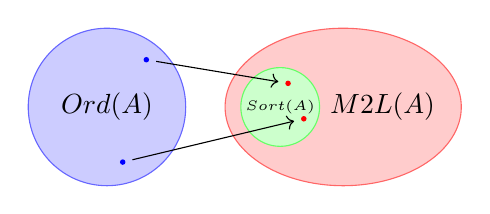
\begin{tikzpicture}
        % draw the sets
        \filldraw[fill=blue!20, draw=blue!60] (-1.5,0) circle (1cm);
        \filldraw[fill=red!20, draw=red!60] (1.5,0) ellipse (1.5cm and 1cm);
        \filldraw[fill=green!20, draw=green!60] (0.7,0) circle (0.5cm);
    
        % the texts
        \node at (-1.5,0) {$\Ord(A)$};
        \node at (0.7, 0) {\tiny$\Sort(A)$};
        \node at (2,0) {$\setmtol(A)$};

    
        % the points in the sets (here I just create nodes to use them later on to position
        % the circles and the arrows
        \node (x1) at (-1,0.6) {};
        \node (x2) at (-1.3,-0.7) {};
        \node (y1) at (0.8,0.3) {};
        \node (y2) at (1,-0.15) {};
    
        % position the elements in the sets (at the nodes we just created)
        \fill[blue] (x1) circle (1pt);
        \fill[blue] (x2) circle (1pt);
        \fill[red] (y1) circle (1pt);
        \fill[red] (y2) circle (1pt);
    
        % draw the arrows
        \draw[->] (x1) -- (y1);
        \draw[->] (x2) -- (y2);
    \end{tikzpicture}
\end{center}

\only<2>{
  This \textit{seems} trivial to prove.

  Construct $\otof(r)$ by parameterizing any sorting algorithm
  by the order relation $r$ and we are done!

  But\dots

  We want to show that there are exactly 6 sorting functions because
  there are exactly 6 orderings.

  $\otof(r)$ should be an isomorphism from $\setord(A)$ to $\setsort(A)$.

  What is the inverse of $\otof(r)$?
}

\end{frame}

\begin{frame}{Introduction}
    Thank you!
\end{frame}

\begin{frame}[standout]
    Thank you!
\end{frame}

% \nocite{*}

\begin{frame}[allowframebreaks]
    \frametitle{References}
    \printbibliography[heading=none]
\end{frame}

\end{document}
